% Generated figures are reconstructed from immutable Experiment006/007
% archives with visuals/render_visual_suite.py and audited source checksums.
\section{Smoothness as relative noise attribution: calibrated simulation evidence}
\label{sec:precision}

\subsection{What the normalized index identifies}
For a third-order difference operator $D=D_3$ and a fixed reference
$\mu$, the model $y=\tau+\varepsilon$,
$D\tau=\mu\mathbf 1+u$, with independent Gaussian disturbances
$\varepsilon\sim N(0,\sigma_\varepsilon^2I)$ and
$u\sim N(0,\sigma_u^2I)$, implies
\begin{equation}
\label{eq:noise-fraction}
\lambda=\frac{\sigma_\varepsilon^2}{\sigma_u^2},
\quad
S(\lambda)=\frac{1}{m}\sum_{j=1}^m
\frac{\lambda\delta_j}{1+\lambda\delta_j},\quad m=n-3.
\end{equation}
On the spectral coordinates of $Dy$, the $j$th summand is the
\emph{fraction of variance due to differenced observation error},
not the fraction of observations that are erroneous. Figure
\ref{fig:precision-spectrum} illustrates these spectral weights and
the exact conditional complexity identity
$\operatorname{df}(H_\lambda)=n-(n-3)S(\lambda)$. This latter identity
holds for a \emph{fixed} reference mean; if $\mu$ is estimated, the
unpenalized effective complexity can increase.

\begin{figure*}[t]
\centering
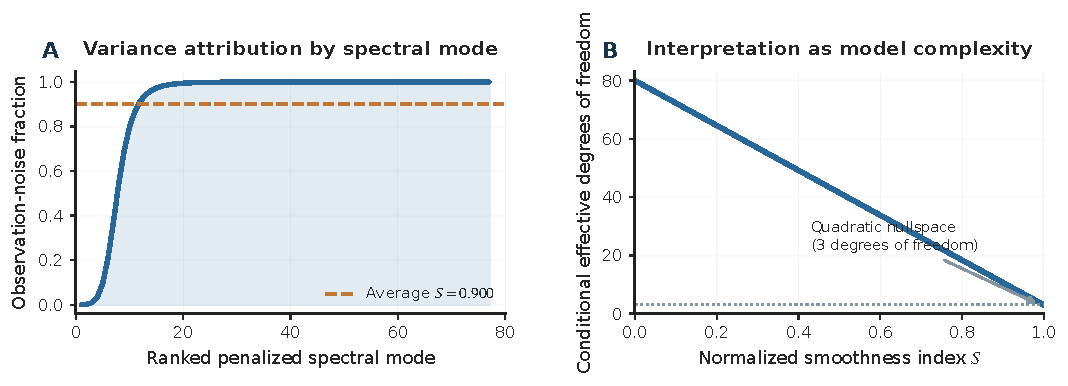
\includegraphics[width=\textwidth]{figures/exp007_spectral_interpretation.pdf}
\caption{Meaning of the normalized $d=3$ smoothness index. (A) Ranked
observation-noise variance fractions in 77 penalized third-difference
spectral directions for $n=80$, $\Delta t=0.1$\,s, observation SD
$0.05$\,m and true jerk innovation SD $2$\,m/s$^3$ under the
independent Gaussian model; their average is $S$. (B) Exact
conditional effective degrees of freedom as a function of $S$ when
the mean of differences is fixed. Neither panel treats $S$ as an
absolute sensor-noise standard deviation.}
\label{fig:precision-spectrum}
\end{figure*}

If observation noise and genuine jerk innovations are correlated
in time, the scalar variance-ratio formula no longer gives the
correct covariance allocation. Nevertheless, the known generative
covariance matrices define a target for validation:
\begin{equation}
\label{eq:noise-cov-fraction}
S_{\mathrm{cov}}
=\frac{1}{n-3}
\operatorname{tr}\!\left[
(C_u+C_\varepsilon)^{-1}C_\varepsilon
\right],
\end{equation}
where $C_u=\operatorname{Cov}(D\tau-\mu\mathbf 1)$ and
$C_\varepsilon=\operatorname{Cov}(D\varepsilon)$.
Under independent Gaussian disturbances Eq.~\eqref{eq:noise-cov-fraction}
equals Eq.~\eqref{eq:noise-fraction} at the true variance ratio.
Under covariance misspecification an estimated $S$ need not
estimate $S_{\mathrm{cov}}$.

\subsection{A known-jerk experiment with paired noise interventions}
We independently manipulate position-measurement noise and the
actual fluctuations of physical jerk. Each of $n=80$ clean
positions is constructed from a prescribed true third difference
$D_3\tau=(\Delta t)^3j$. Experimental levels are three
observation-noise standard deviations ($0.01,0.05,0.20$\,m)
and three jerk-innovation standard deviations
($0.5,2,8$\,m/s$^3$). We cross these with independent, AR(1),
and terminal-contaminated measurement errors, and with independent,
AR(1), and abrupt-reversal jerk processes. The terminal outlier
has randomized sign, so its mixture covariance is known, but
the observations are not Gaussian. The reversal violates the
constant jerk-reference assumption.

The frozen confirmatory design has $1{,}944$ factorial cases
and four smoothing selectors per case. \emph{Only 72 independent
parent random draws underlie the 1,944 cases}: standardized jerk
innovations and measurement-error draws are held constant across
all 27 treatments within each parent. The $162$-case pilot uses
a separate seed namespace. All $7{,}776$ confirmatory fits were
valid. The four selectors are Gaussian profile likelihood with
the known generative $\mu$ (a simulation-only control), unknown-mean
Gaussian REML, conditional profile likelihood with noisy global
cubic OLS $\widehat\mu$, and zero-mean GCV on the original 15-point
smoothness grid.

\begin{figure*}[t]
\centering
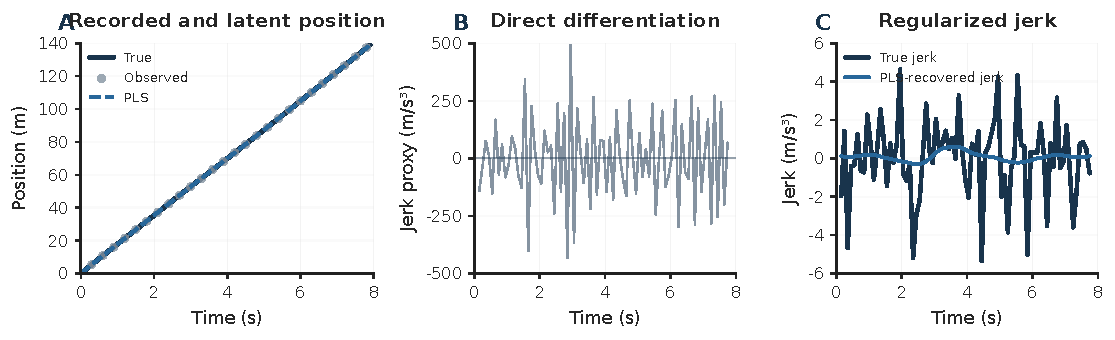
\includegraphics[width=\textwidth]{figures/exp007_jerk_example.pdf}
\caption{One \emph{predeclared} analytic trajectory from the
independent Gaussian regime (confirmation trial 000010;
observation SD $0.05$\,m, jerk-innovation SD $2$\,m/s$^3$).
(A) Prescribed clean position, noisy observations and
PLS fit using global cubic OLS $\widehat\mu$ and profiled
Gaussian likelihood; (B) the raw third difference divided
by $(0.1\,\mathrm{s})^3$, with severe noise amplification;
(C) known prescribed jerk and the PLS-reconstructed third
difference. The raw and regularized jerk panels have
different vertical scales. This generated example is
\emph{not} a claimed independent real NGSIM jerk measurement.}
\label{fig:precision-jerk}
\end{figure*}

\subsection{Calibration and independent changes in noise and jerk}
Under the correctly specified independent Gaussian model,
unknown-mean REML produced Spearman correlation $0.965$
between selected $S$ and the true spectral noise fraction,
with absolute calibration error $0.0115$ averaged over the
216 paired factor combinations (24 stochastic parents).
The known-reference control achieved $0.967$ and $0.0107$,
respectively, while the global cubic OLS plug-in achieved
$0.966$ and $0.0143$. The zero-reference GCV comparator
achieved $0.901$ and $0.0249$. These are \emph{descriptive}
correlations over dependent factorial cases, not independent
sample significance tests.

\begin{figure*}[t]
\centering
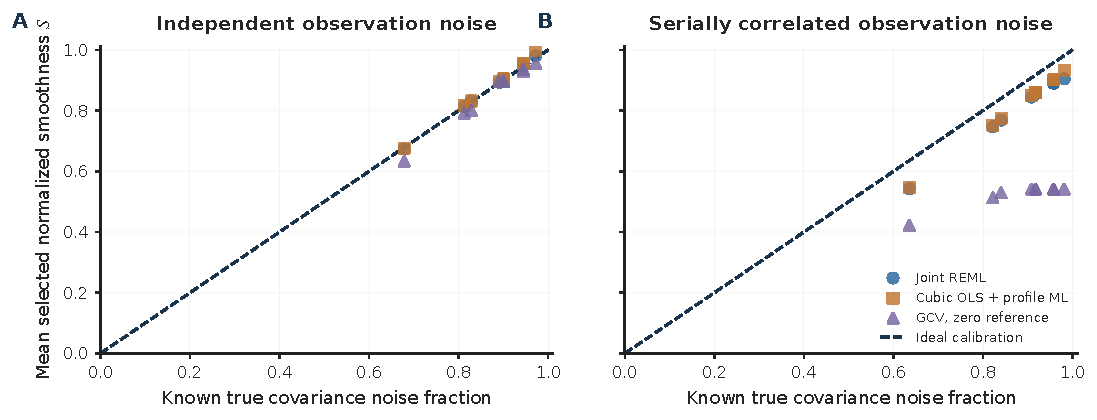
\includegraphics[width=\textwidth]{figures/exp007_calibration.pdf}
\caption{Empirical calibration of the selected smoothness
coordinate against the \emph{true covariance-based} noise fraction.
Each point aggregates 24 independent parents at one of nine
observation-noise/jerk-volatility combinations; three practical
selectors are shown. (A) Independent observation noise and
independent jerk innovations. (B) Correlated AR(1) observation
noise with otherwise independent jerk innovations: rank
association persists, but calibrated values systematically
depart from the identity line. An oracle known-$\mu$ control
is excluded from this practical-selection visualization.}
\label{fig:precision-calibration}
\end{figure*}

For unknown-mean REML under independent Gaussian errors,
raising position-noise SD from $0.01$ to $0.20$\,m at
fixed jerk SD increased fitted $S$ by $0.1498$
(known theoretical increase $0.1451$). Raising actual jerk
innovation SD from $0.5$ to $8$\,m/s$^3$ at fixed observation
noise \emph{decreased} fitted $S$ by $0.1387$
(known theoretical decrease $0.1337$). Paired parent-level
bootstrap intervals were $[0.1454,0.1544]$ and
$[-0.1428,-0.1345]$, respectively, conditional on this
particular simulation design. Figure~\ref{fig:precision-effects}
shows the corresponding results across all nine covariance
and maneuver regimes, including the less accurate
misspecified cases.

\begin{figure*}[t]
\centering
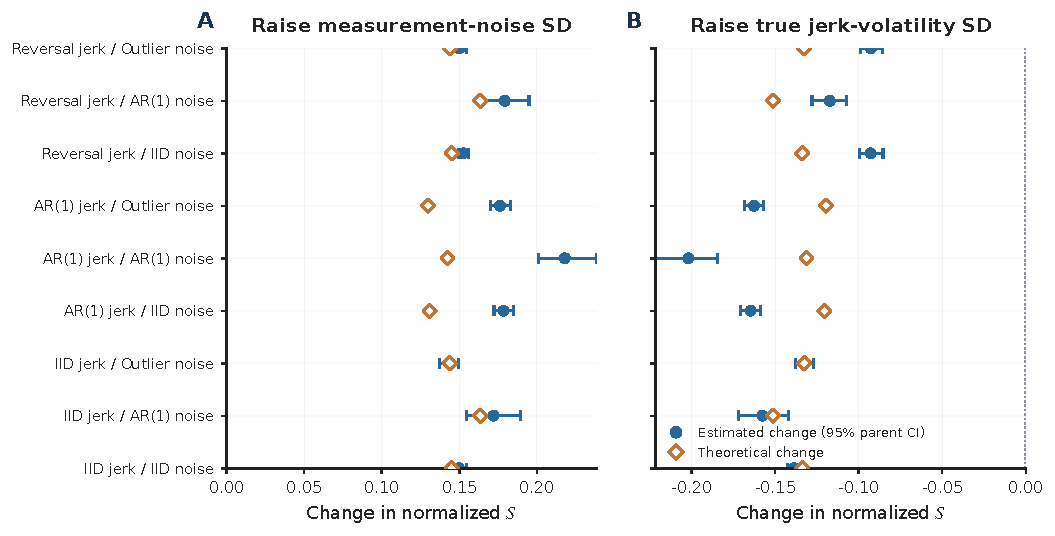
\includegraphics[width=\textwidth]{figures/exp007_interventions.pdf}
\caption{Two separately controlled interventions for selected
joint-REML smoothness across nine jerk/measurement-error
structures. (A) Increasing observation-noise SD with true jerk
volatility fixed; (B) increasing true jerk volatility with
observation noise fixed. Blue circles and whiskers show
parent-cluster means and 95\% Monte Carlo bootstrap intervals;
open orange diamonds are known covariance-theoretic effects.
Theoretical effects vary by correlation regime. Paired factor
combinations within each independent parent are never
resampled as independent observations.}
\label{fig:precision-effects}
\end{figure*}

A direct identifiability counterexample prevents interpreting
$S$ as \emph{absolute measurement precision}: increasing
$(\sigma_\varepsilon,\sigma_j)$ from
$(0.05\ \mathrm{m},2\ \mathrm{m/s^3})$ to
$(0.20\ \mathrm{m},8\ \mathrm{m/s^3})$ preserves the
variance ratio and therefore $S$ under the independent
Gaussian model, even though the observation-noise variance
increases sixteenfold. The same-ratio experiment produced
an estimated mean $\Delta S$ statistically indistinguishable
from zero by design. The index is relative to dynamical
innovation variation, not a stand-alone metrological rating
of recording quality.

\subsection{Where the precision interpretation fails}
Figure~\ref{fig:precision-robustness} displays calibration
errors under deliberately misspecified noise and dynamics.
For joint REML, mean absolute error increased from $0.0115$
under independent Gaussian disturbances to $0.0712$
when the measurement error had AR(1) correlation of $0.65$,
and to $0.1111$ when both the measurement noise and jerk
innovations were serially correlated. Hence favorable rank
correlation alone is insufficient to claim quantitatively
accurate noise attribution.

\begin{figure*}[t]
\centering
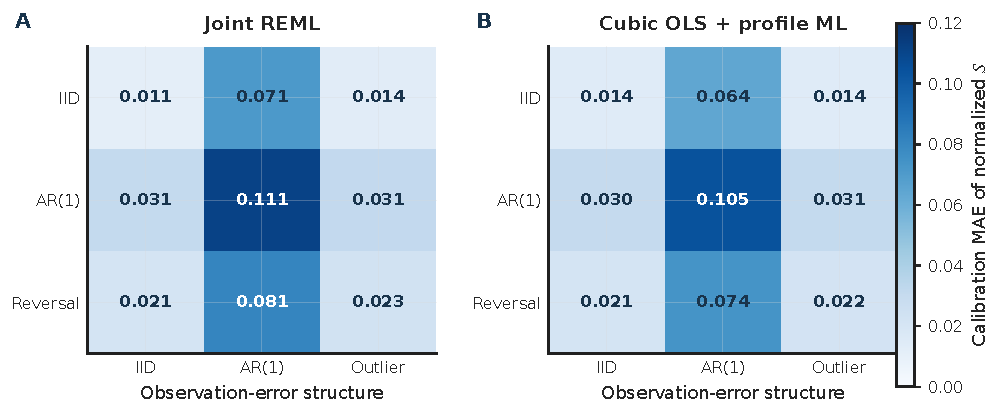
\includegraphics[width=\textwidth]{figures/exp007_misspecification.pdf}
\caption{Absolute $S$ calibration error against the
\emph{known} covariance-noise fraction, by true jerk structure
(rows) and observation-error structure (columns). Left:
properly mean-adjusted joint REML; right: global cubic
OLS reference followed by fixed-mean Gaussian profile
likelihood. The independently Gaussian regime occupies the
upper-left cell. Darker values indicate larger errors;
the AR(1) observation-error cases are conspicuous failures
of the independent-noise statistical model.}
\label{fig:precision-robustness}
\end{figure*}

\subsection{Precision calibration is not jerk or forecast optimality}
The preceding calibration evidence does not imply that
unknown-mean REML minimizes jerk reconstruction or
future-position loss. In a separate frozen known-jerk
Experiment006 ($1{,}296$ confirmation trials), a global
cubic OLS reference followed by continuous profile
likelihood attained $2.441$\,m/s$^3$ historical discrete-jerk
RMSE, compared with $3.295$\,m/s$^3$ for joint REML.
Conversely, when forecasting \emph{clean synthetic} position
one second ahead using the 25-point continuation, a fixed
zero reference and continuous Gaussian profile ML attained
$0.405$\,m RMSE versus $0.498$\,m for joint REML.

For a different group of $200$ real NGSIM recorded episodes,
a GCV-selected natural cubic smoothing spline with quadratic
Taylor continuation attained $0.348$\,m pooled one-second
recorded-position RMSE, better than joint REML with the
25-point continuation ($0.578$\,m). On these real episodes
the continuous joint-REML selector chose the unsmoothed
$\lambda\to0$ covariance boundary in $161/200$ cases:
this is an important boundary warning, \emph{not}
evidence of precisely observed jerk. Figure
\ref{fig:precision-endpoints} compares the distinct
physical and forecast targets rather than treating all
errors as interchangeable.

\begin{figure*}[t]
\centering
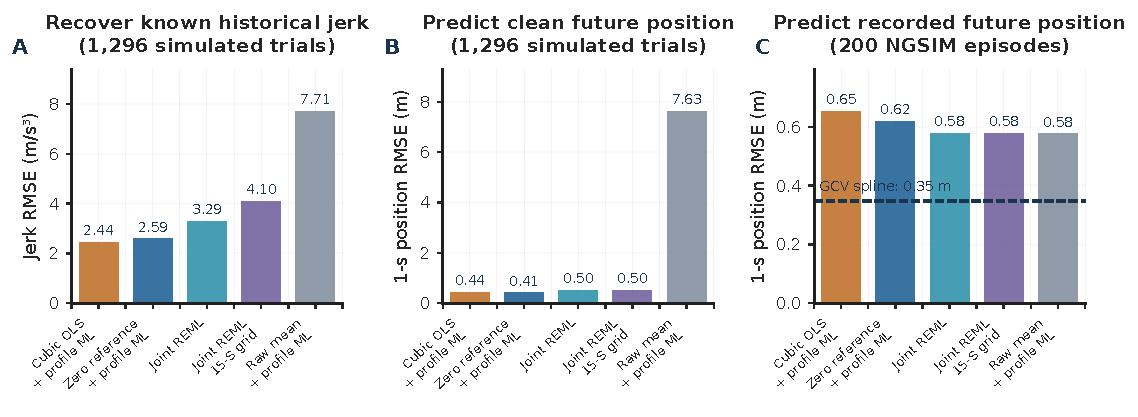
\includegraphics[width=\textwidth]{figures/exp006_reconstruction_forecasting.pdf}
\caption{Different estimation targets favor different PLS
reference and smoothing policies. (A) Known historical
discrete jerk RMSE across 1,296 analytic synthetic
trajectories. (B) One-second future \emph{clean} position
RMSE on those same synthetic trajectories using the
25-point continuation. (C) One-second \emph{recorded}
future position RMSE on 200 real NGSIM episodes, with
the corresponding GCV smoothing-spline benchmark shown
as a dashed horizontal line. Smaller is better within
each panel. The three panels have different response
units or targets and do not constitute one common metric.}
\label{fig:precision-endpoints}
\end{figure*}

The controlled calibration and real-data comparisons
therefore support a \emph{conditional and interpretable}
smoothing coordinate, not a universal sensor-quality
index or general forecasting advantage. All synthetic
source trajectories, selection rows, bootstrap draws,
figure scripts and full file SHA-256 inventories are
preserved in the isolated Experiment006 and Experiment007
Git results branches and the university Windows runner.
